\documentclass[aspectratio=169,11pt,t]{beamer}
% ============================================================
%  ksa-cs-v2: ksa-cs-lecture-template.tex 스타일 + 한글, v2 덱(16:9)용.
%    - 짙은 네이비 헤드라인 (섹션 이름 + 프레임마다 점)
%    - 꽉 찬 파란 제목 막대, 둥근 그림자 블록
%    - 한글: Noto Sans CJK KR (fontspec)
%  사용:
%    \documentclass[aspectratio=169,11pt,t]{beamer}
%    \input{<..>/theme/ksa-cs-v2.tex}
%  ksa-theme.tex 의 매크로(\kb \kq, ksablue/ksared 등)도 같은 이름으로 둔다
%  -> v2 덱 본문을 거의 그대로 옮길 수 있다.
% ============================================================

\usepackage{fontspec}
\usepackage{amsmath,amssymb}
\usepackage{tikz}
\usepackage{listings}
\usepackage{graphicx}
\usepackage{booktabs}
\usepackage{varwidth}
% enumitem 은 넣지 않는다 (beamer 글머리표가 사라진다)

\defaultfontfeatures{Ligatures=TeX}
\setmainfont{Noto Sans CJK KR}
\setsansfont{Noto Sans CJK KR}
\setmonofont{Noto Sans Mono CJK KR}[Scale=0.92]
\usefonttheme{professionalfonts}

% ---------- 기본 틀 ----------
\usetheme{default}
\useinnertheme[shadow=true]{rounded}
\setbeamertemplate{navigation symbols}{}
\setbeamersize{text margin left=1em,text margin right=1em}

% ---------- 색 (템플릿 원본 값) ----------
\definecolor{navydark}{HTML}{191959}
\definecolor{navydim}{HTML}{8888B0}
\definecolor{navytitle}{HTML}{262686}
\definecolor{navyblue}{HTML}{3333B2}
\definecolor{blockbodybg}{HTML}{E9E9F3}
\definecolor{examplegreen}{HTML}{006000}
\definecolor{examplebg}{HTML}{E5EFE5}
\definecolor{alertred}{HTML}{BF0000}
\definecolor{alertbg}{HTML}{F9E5E5}
% ksa-theme.tex 와 같은 이름 (본문 호환)
\colorlet{ksablue}{navytitle}
\colorlet{ksabluedk}{navydark}
\definecolor{ksagold}{HTML}{D6CBB1}
\definecolor{ksagolddk}{HTML}{A9976B}
\colorlet{ksared}{alertred}
\definecolor{ksagray}{HTML}{5B5B5B}

\setbeamercolor{structure}{fg=navyblue}
\setbeamercolor{alerted text}{fg=alertred}
\setbeamercolor{frametitle}{bg=navytitle,fg=white}
\setbeamercolor{title}{fg=white,bg=navytitle}
\setbeamercolor{block title}{bg=navytitle,fg=white}
\setbeamercolor{block body}{bg=blockbodybg,fg=black}
\setbeamercolor{block title example}{bg=examplegreen,fg=white}
\setbeamercolor{block body example}{bg=examplebg,fg=black}
\setbeamercolor{block title alerted}{bg=alertred,fg=white}
\setbeamercolor{block body alerted}{bg=alertbg,fg=black}
\setbeamercolor{item}{fg=navyblue}
\setbeamertemplate{itemize item}[circle]
\setbeamertemplate{itemize subitem}[triangle]

% ---------- 헤드라인: miniframes (섹션 이름 + 점) ----------
\useoutertheme[subsection=false]{miniframes}
\setbeamerfont{section in head/foot}{size=\tiny}
\setbeamercolor{section in head/foot}{bg=navydark,fg=white}
\setbeamercolor{mini frame}{fg=white}
\setbeamertemplate{mini frames}[circle]

% ---------- 제목 막대: 폭 꽉 채움, 두 줄까지 ----------
\setbeamerfont{frametitle}{size=\normalsize,series=\bfseries}
\setbeamertemplate{frametitle}{%
  \nointerlineskip
  \begin{beamercolorbox}[wd=\paperwidth,ht=2.7ex,dp=1.1ex,leftskip=.3cm,rightskip=.3cm]{frametitle}%
    \usebeamerfont{frametitle}\insertframetitle
  \end{beamercolorbox}}

% ---------- 쪽 번호: 오른쪽 아래 ----------
\setbeamertemplate{footline}{%
  \hfill
  {\color{navydim}\scriptsize\insertframenumber\,/\,\inserttotalframenumber}%
  \hspace{3mm}\vspace{2mm}%
}

% ---------- 표지: 템플릿처럼 헤드라인은 그대로, 가운데 둥근 그림자 상자에 제목 한 줄 ----------
% 덱에서:  {\setbeamertemplate{footline}{}\begin{frame}[c,noframenumbering]\titlepage\end{frame}}
\setbeamercolor{title}{fg=white,bg=navyblue}
\makeatletter
\setbeamertemplate{title page}{%
  \vfill
  \centering
  \begin{minipage}{0.84\paperwidth}
  \begin{beamercolorbox}[wd=\linewidth,sep=7pt,center,rounded=true,shadow=true]{title}
    {\usebeamerfont{title}\inserttitle\par}%
    \ifx\insertsubtitle\@empty\else\vskip0.4em{\usebeamerfont{subtitle}\insertsubtitle\par}\fi
  \end{beamercolorbox}
  \end{minipage}\par\vskip1.6em
  {\usebeamerfont{author}\color{navytitle}\insertauthor\par}\vskip0.3em
  {\usebeamerfont{institute}\color{ksagray}\insertinstitute\par}
  \vfill
}
\makeatother
\setbeamerfont{title}{series=\bfseries,size=\Large}
\setbeamerfont{subtitle}{size=\normalsize}
\setbeamerfont{author}{size=\normalsize}
\setbeamerfont{institute}{size=\small}

% ksa-theme 호환: 덱이 \renewcommand{\ksacredit}{..} 를 해도 되게 (꼬리말에는 안 쓴다)
\newcommand{\ksacredit}{}

% ---------- 강조 ----------
\newcommand{\hl}[1]{\textcolor{alertred}{#1}}
\newcommand{\hlb}[1]{\textcolor{navyblue}{#1}}
\newcommand{\kb}[1]{\textbf{\color{ksablue}#1}}
\newcommand{\kq}[1]{\textbf{\color{ksared}#1}}

% ---------- 파이썬 코드 (템플릿과 같은 색) ----------
\definecolor{codekw}{HTML}{0033B3}
\definecolor{codebuiltin}{HTML}{BF0000}
\definecolor{codestr}{HTML}{067D17}
\definecolor{codecomment}{HTML}{8C8C8C}
\definecolor{codenum}{HTML}{1750EB}
\lstdefinestyle{py}{
  language=Python, basicstyle=\ttfamily\scriptsize,
  keywordstyle=\color{codekw}\bfseries, stringstyle=\color{codestr},
  commentstyle=\color{codecomment}\itshape, numberstyle=\color{codenum},
  emph={print,len,range,sum,input,int,str,float,list,dict,append,remove,sorted,abs,min,max},
  emphstyle=\color{codebuiltin}, showstringspaces=false, keepspaces=true,
  columns=fixed, basewidth=0.52em, aboveskip=1mm, belowskip=1mm, xleftmargin=2mm,
  breaklines=true
}
\lstset{style=py}

% 원본 덱 (ksa-theme): slides/v2/ml1/week03/gaussian/ -- 그림은 거기 figs/ 를 그대로 쓴다
\setbeamerfont{author}{size=\normalsize}
\setbeamerfont{institute}{size=\small}
% t 분포 그림(ga_t_*)은 이 폴더의 make_figs.py -> figs/
\graphicspath{{figs/}{../../../v2/ml1/week03/gaussian/figs/}{../../../assets/}}
\makeatletter
\newcommand{\markpage}[1]{\protected@write\@auxout{}{\string\newlabel{#1}{{\the\c@framenumber}{}}}\hypertarget{#1}{}}
\newcommand{\pref}[1]{\hyperlink{#1}{\textcolor{ksagolddk}{(p.\ref{#1})}}}
\makeatother

\renewcommand{\ksacredit}{Machine Learning and Deep Learning \,\textperiodcentered\, 분포 함수}
\title{분포 함수 (Distribution Functions)}
\subtitle{가우시안 · 스튜던트 t · 푸아송 분포, 그리고 베이즈 분류까지}
\author{Machine Learning and Deep Learning}
\institute{한국과학영재학교 (KSA)}
\date{}
\begin{document}
{\setbeamertemplate{footline}{}\begin{frame}[c,noframenumbering]\titlepage\end{frame}}

\section{질문}
% --- 오늘의 질문
\begin{frame}{오늘의 질문}
\vfill
\begin{columns}[c]
\begin{column}{0.42\textwidth}\centering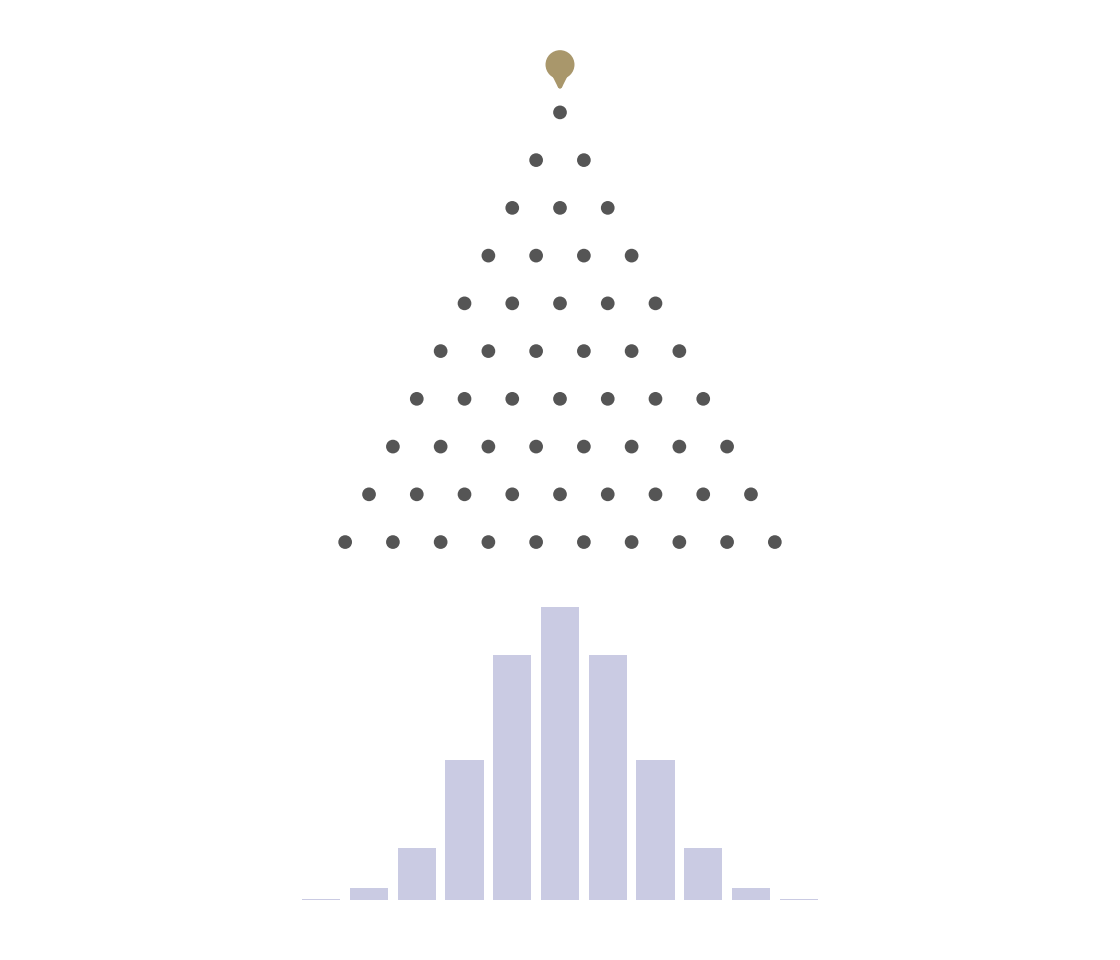
\includegraphics[width=0.95\linewidth]{ga_board.png}\end{column}
\begin{column}{0.54\textwidth}
{\Large 못이 10줄 박힌 판}\\[0.6em]
{\large 공은 못을 만날 때마다\\ 왼쪽 · 오른쪽으로 \textbf{반반} 튄다}\\[1em]
{\Large 공 1000개를 떨어뜨리면\\ \kq{어디에 가장 많이 쌓일까?}}
\end{column}
\end{columns}
\vfill
\note{못이 10줄 박힌 판에 위에서 공을 떨어뜨립니다. 공은 못을 만날 때마다 왼쪽이나 오른쪽으로 반반의 확률로 튑니다. 이 판을 처음 만든 사람의 이름을 따서 골턴 보드라고 부릅니다. 공 1000개를 떨어뜨리면 아래 칸들 중 어디에 가장 많이 쌓일까요? 그리고 쌓인 모양은 어떨까요?}
\end{frame}

\section{종 모양}
% --- 결과
\begin{frame}{가운데 246개, 양 끝 1개}
\markpage{bins}
\vfill
\centering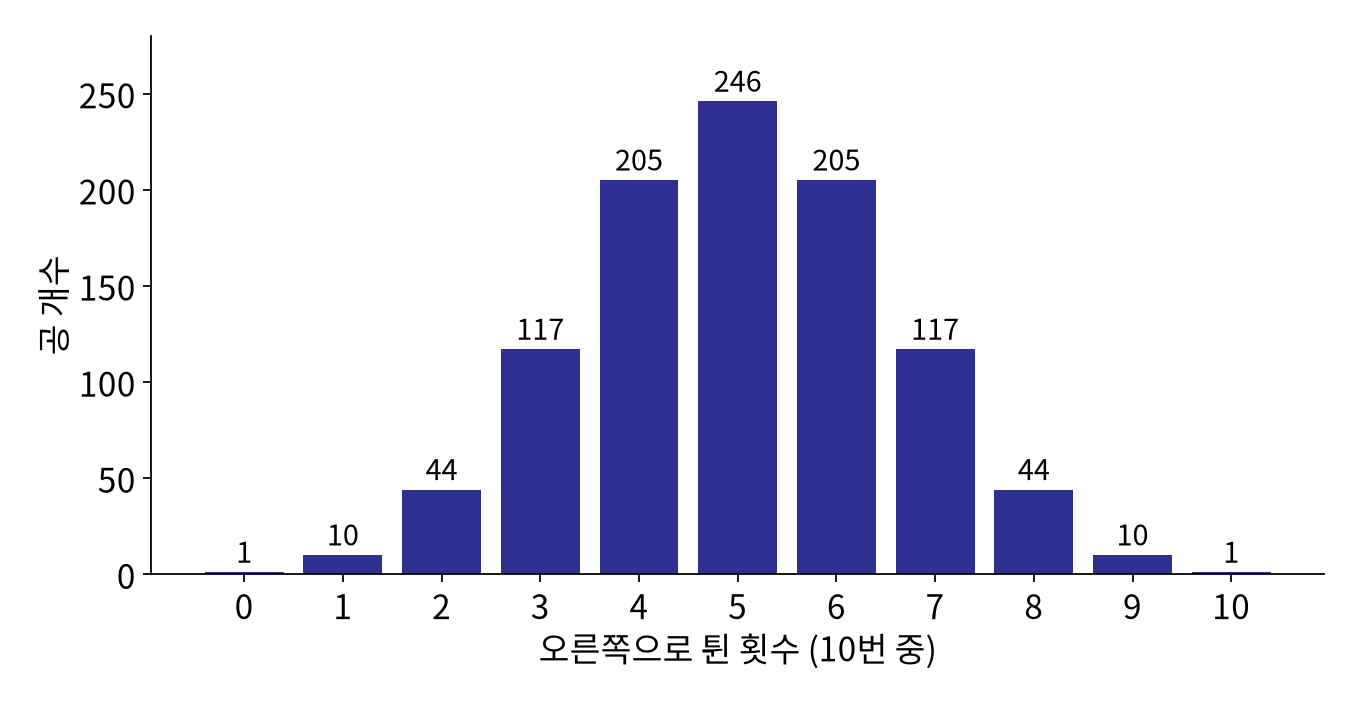
\includegraphics[width=0.62\linewidth]{ga_bins.png}\par\vskip0.2em
{\large 오른쪽으로 $k$번 튀는 길의 수 $= \binom{10}{k}$ \qquad 공 개수 $\approx 1000 \times \dfrac{\binom{10}{k}}{2^{10}}$}
\vfill
\note{결과입니다. 가운데 칸에 246개, 양 끝 칸에는 겨우 1개씩 쌓입니다. 이유는 길의 수입니다. 공이 맨 오른쪽 끝에 가려면 10번 모두 오른쪽으로 튀어야 하는데, 그런 길은 딱 하나입니다. 가운데에 가려면 10번 중 5번만 오른쪽이면 되고, 그런 길은 10개 중 5개를 고르는 경우의 수, 252가지입니다. 길은 모두 2의 10제곱, 1024가지이고 길마다 확률이 같으니, 1000 곱하기 252 나누기 1024가 약 246개입니다.}
\end{frame}

% --- 작은 효과의 합
\begin{frame}{작은 효과가 많이 더해지면 종 모양}
\vfill
\centering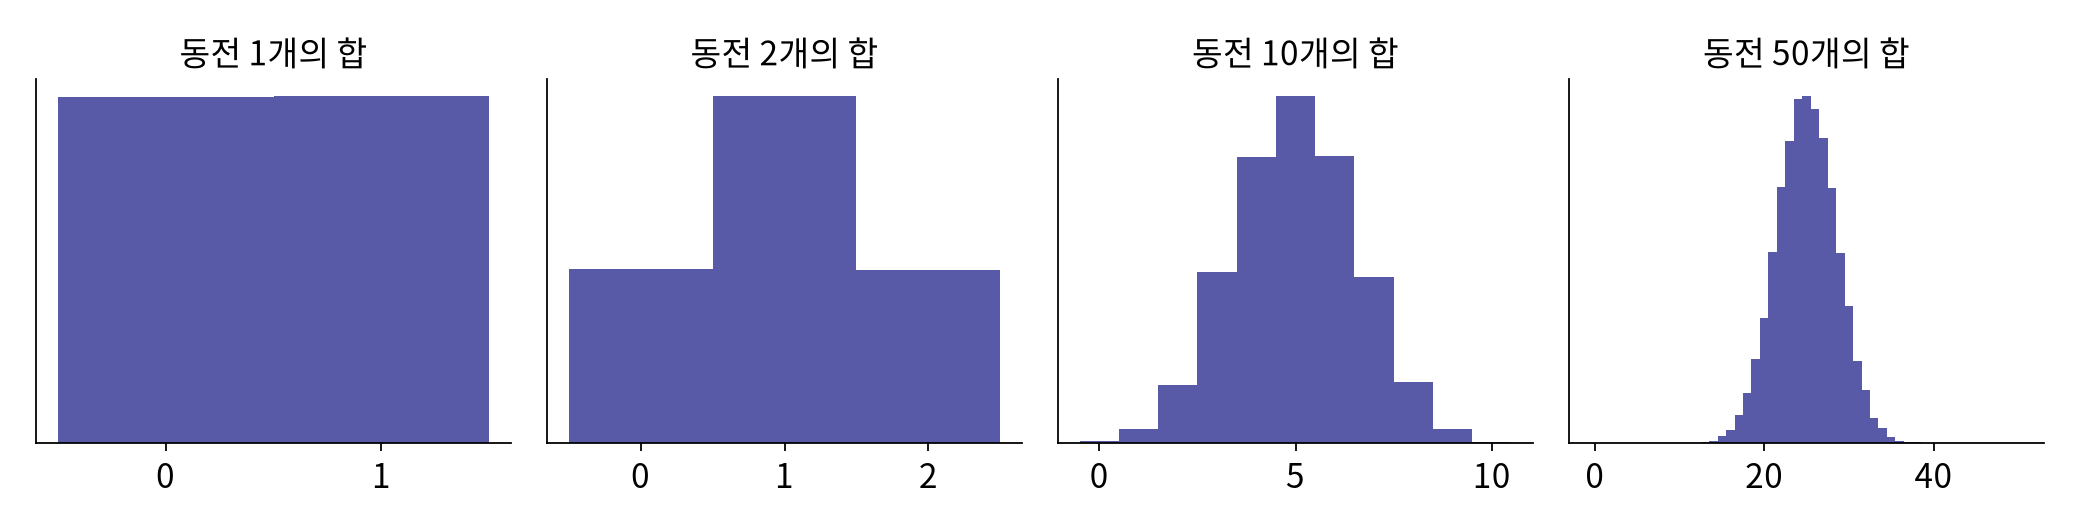
\includegraphics[width=0.96\linewidth]{ga_sum.png}\par\vskip0.3em
{\large 동전(0 또는 1)을 여러 개 더할수록 \kb{종 모양}에 가까워진다}\\[0.3em]
{\small 키 (유전자 수백 개 + 영양 + …), 측정 오차, 시험 점수 $\to$ 작은 효과 여럿의 합이라 종 모양이 흔하다 (중심극한정리)}
\vfill
\note{골턴 보드의 공 위치는 왼쪽이면 0, 오른쪽이면 1인 동전 10개를 더한 것과 같습니다. 동전 하나는 0과 1 두 막대뿐이지만, 2개, 10개, 50개를 더할수록 모양이 점점 매끈한 종 모양이 됩니다. 이 종 모양을 가우시안 분포, 또는 정규분포라고 부릅니다. 자연에서 종 모양이 흔한 이유가 여기 있습니다. 키는 수백 개의 유전자와 영양 같은 작은 효과의 합이고, 측정 오차도 여러 작은 오차의 합입니다. 작은 독립적인 효과가 많이 더해지면 종 모양이 된다는 사실을 중심극한정리라고 합니다.}
\end{frame}

\section{가우시안}
% --- 식
\begin{frame}{가우시안 분포: 숫자 두 개로 정해진다}
\markpage{pdf}
\vfill
\centering
{\LARGE\[ p(x) = \frac{1}{\sqrt{2\pi}\,\sigma}\exp\!\left(-\frac{(x-\textcolor{ksablue}{\mu})^2}{2\textcolor{ksared}{\sigma}^2}\right) \]}\vskip0.6em
\renewcommand{\arraystretch}{1.3}
{\large\begin{tabular}{lll}
\textcolor{ksablue}{$\mu$} & 평균 (mean) & 종의 가운데\\
\textcolor{ksared}{$\sigma$} & 표준편차 (standard deviation) & 종이 퍼진 정도 \quad ($\sigma^2$: 분산)\\
$\frac{1}{\sqrt{2\pi}\sigma}$ & 높이 맞춤 & 전체 넓이가 1 이 되게
\end{tabular}}\vskip0.4em
{\small 줄여서 $\mathcal{N}(\mu, \sigma^2)$ 로 쓴다}
\vfill
\note{가우시안 분포의 식입니다. 복잡해 보이지만 정하는 숫자는 두 개뿐입니다. 파란 뮤는 평균으로 종의 가운데 위치, 빨간 시그마는 표준편차로 종이 퍼진 정도입니다. 시그마 제곱은 분산이라고 부릅니다. 지수 안을 보면 x가 뮤에서 멀어질수록 제곱으로 작아지고, 시그마가 클수록 천천히 작아집니다. 앞의 상수는 전체 넓이가 1이 되도록, 즉 확률이 되도록 높이를 맞춰 주는 숫자입니다. 이 분포를 줄여서 N 뮤 시그마 제곱이라고 씁니다.}
\end{frame}

% --- 바꿔 보기
\begin{frame}{$\mu$ 는 위치, $\sigma$ 는 폭}
\vfill
\centering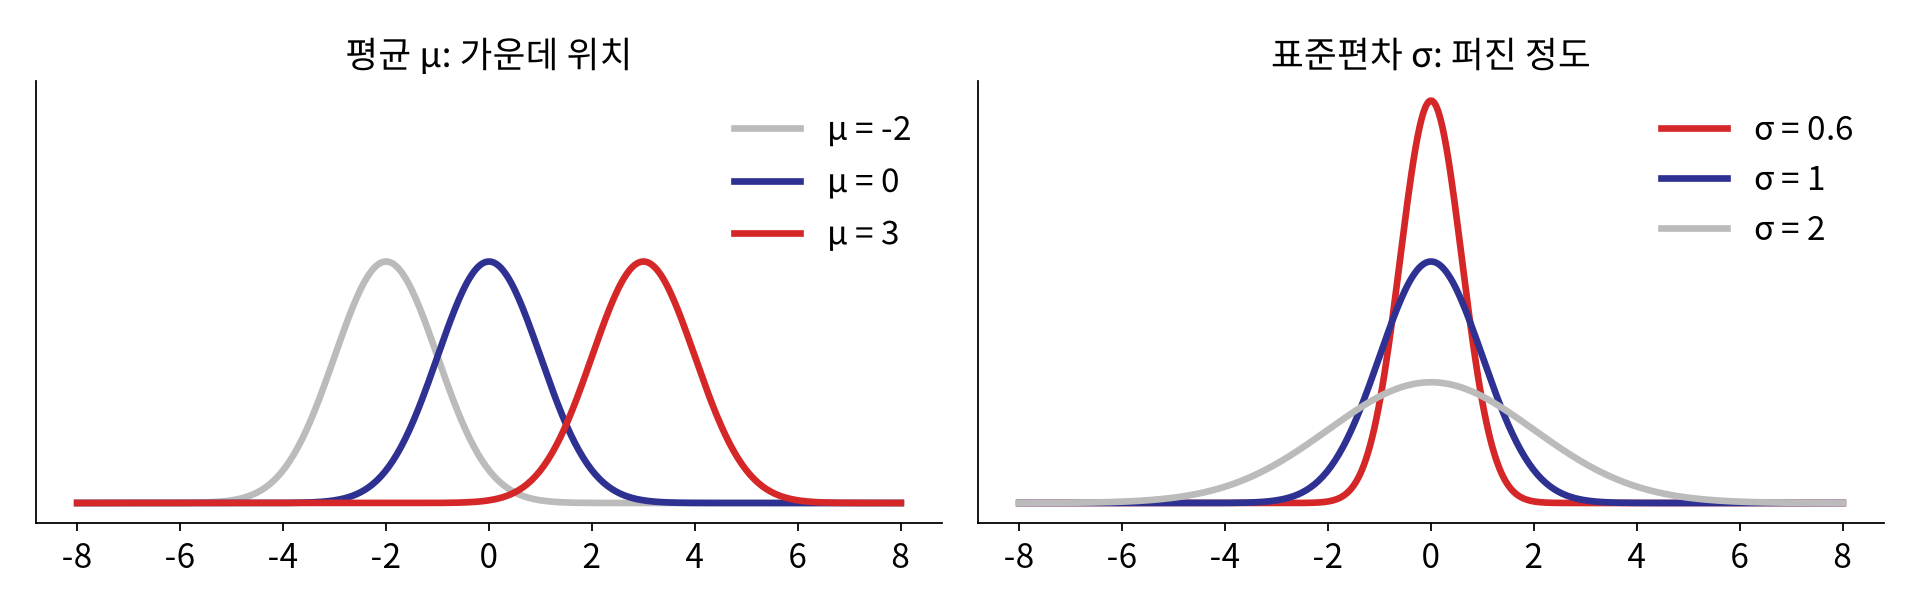
\includegraphics[width=0.9\linewidth]{ga_musd.png}\par\vskip0.3em
{\large $\mu$: 종이 \kb{옆으로 이동} \qquad $\sigma$ 를 키우면 \kq{낮고 넓게} (넓이는 항상 1)}
\vfill
\note{뮤를 바꾸면 종 모양은 그대로 옆으로 움직입니다. 시그마를 키우면 종이 낮고 넓게 퍼지고, 줄이면 높고 좁아집니다. 전체 넓이는 항상 1이니까, 넓게 퍼지면 그만큼 낮아질 수밖에 없습니다.}
\end{frame}

% --- 68 95
\begin{frame}{평균에서 $\sigma$ 1개 안에 68\%, 2개 안에 95\%}
\markpage{rule}
\vfill
\centering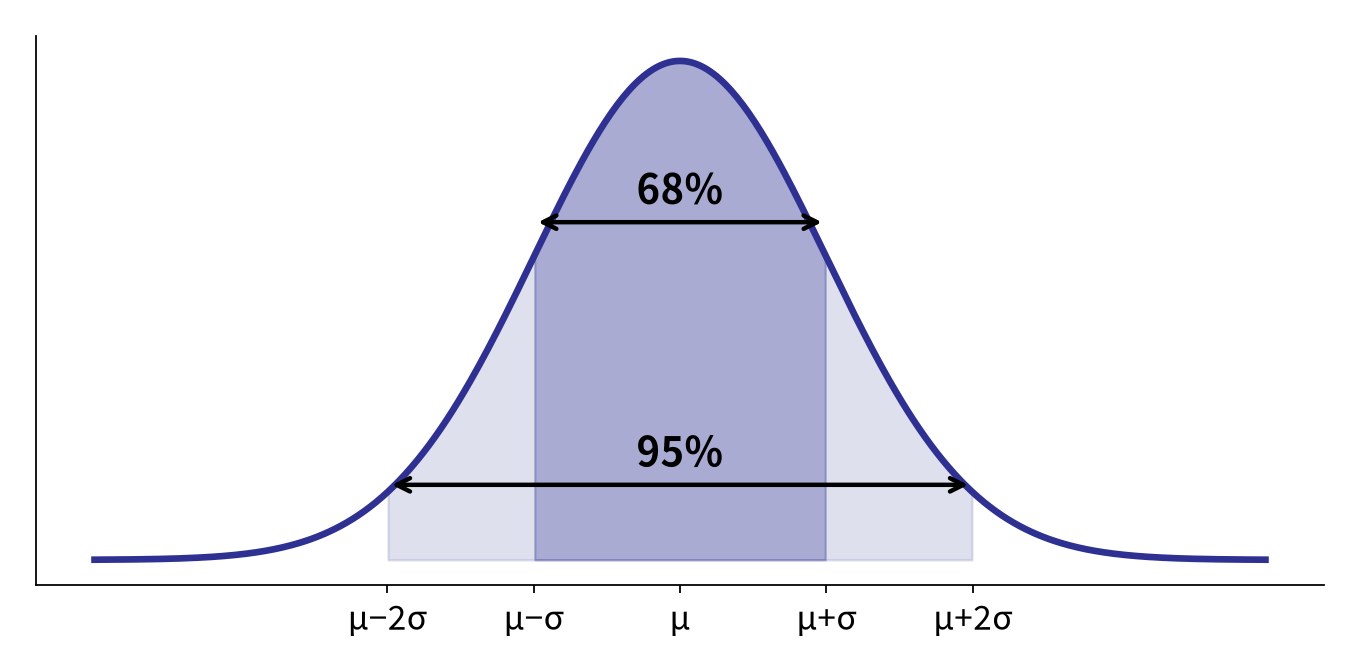
\includegraphics[width=0.62\linewidth]{ga_6895.png}\par\vskip0.3em
{\large 어떤 $\mu$, $\sigma$ 든 같다 \qquad $\pm 3\sigma$ 안에는 99.7\%}
\vfill
\note{가우시안 분포에는 유용한 규칙이 있습니다. 평균에서 표준편차 1개만큼 양쪽으로 가면 그 안에 전체의 68퍼센트가 들어옵니다. 2개만큼이면 95퍼센트, 3개면 99.7퍼센트입니다. 뮤와 시그마가 무엇이든 똑같이 성립합니다. 그래서 표준편차 단위로 생각하면 어떤 가우시안이든 같은 말로 이야기할 수 있습니다.}
\end{frame}

% --- 시험
\begin{frame}{평균 70, 표준편차 10 인 시험에서 90점 이상은?}
\vfill
\centering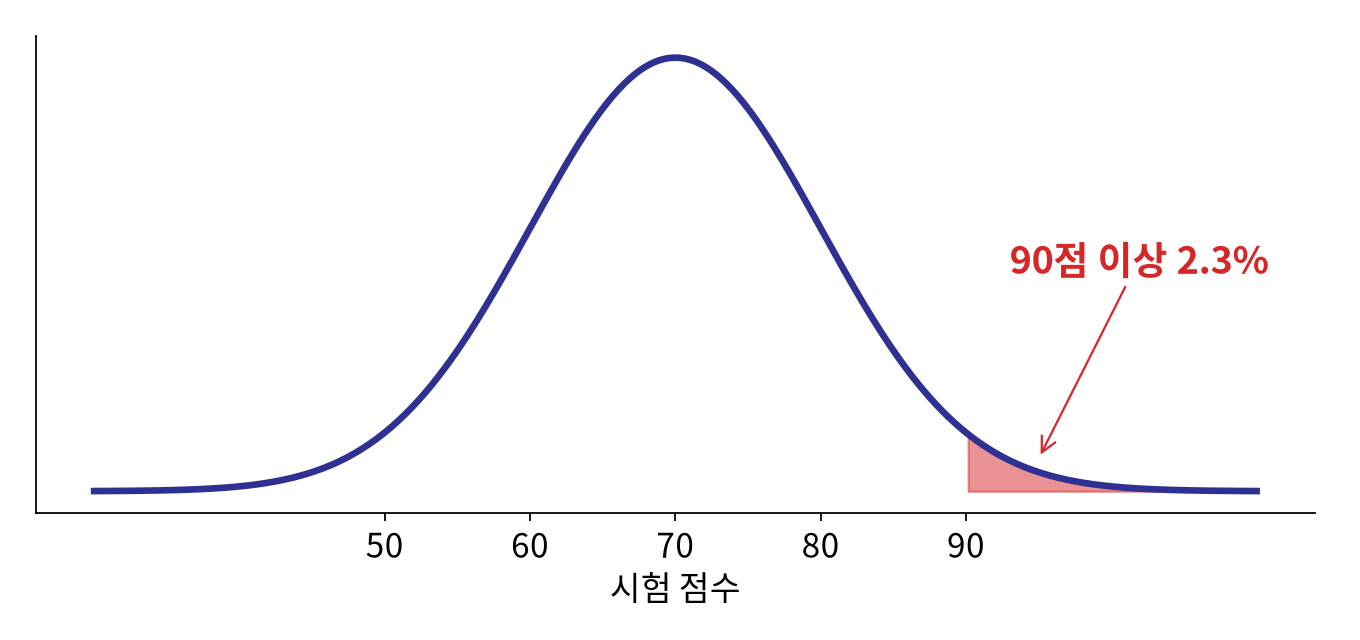
\includegraphics[width=0.56\linewidth]{ga_exam.png}\par\vskip0.2em
{\Large\[ z = \frac{x - \mu}{\sigma} = \frac{90 - 70}{10} = 2 \]}
{\large 평균에서 $\sigma$ 2개 위 \quad $\to$ \quad 95\% 밖의 한쪽 절반 $\approx$ \kq{2.3\%}}
\vfill
\note{평균 70점, 표준편차 10점인 시험에서 90점 이상은 몇 퍼센트일까요? 90점이 평균에서 표준편차 몇 개만큼 떨어져 있는지를 보면 됩니다. 90 빼기 70을 10으로 나누면 2, 이 값을 z 점수라고 합니다. 평균에서 2시그마 안에 95퍼센트가 있으니 밖은 5퍼센트이고, 위쪽과 아래쪽에 반씩이니 위쪽은 약 2.5퍼센트입니다. 정확히 계산하면 2.3퍼센트입니다. 100명 중 두세 명꼴입니다.}
\end{frame}

% --- 데이터에서 구하기
\begin{frame}{데이터에서 $\mu$, $\sigma$ 구하기}
\markpage{fit}
\vfill
\centering
{\large 키 5명: \; 168, 172, 174, 176, 180 cm}\vskip0.6em
{\large\[ \hat\mu = \frac{1}{m}\sum_{i=1}^{m} x^{(i)} = \frac{870}{5} = 174 \]
\[ \hat\sigma^2 = \frac{1}{m}\sum_{i=1}^{m}\big(x^{(i)} - \hat\mu\big)^2 = \frac{36 + 4 + 0 + 4 + 36}{5} = 16 \]}\vskip0.4em
{\large $\hat\sigma = 4$ cm \qquad $\to$ \quad 이 데이터를 가장 잘 설명하는 종 $= \mathcal{N}(174,\ 4^2)$}\\[0.4em]
{\small 데이터가 나올 확률(가능도)을 가장 크게 하는 값 (최대가능도 추정, MLE) \quad $\hat\mu$: 데이터로 추정한 값}
\vfill
\note{실제 데이터에서 뮤와 시그마는 어떻게 구할까요? 키 5명의 데이터가 있습니다. 뮤는 그냥 평균, 870을 5로 나눈 174입니다. 시그마 제곱은 평균에서 떨어진 거리의 제곱을 평균 낸 것입니다. 마이너스 6, 마이너스 2, 0, 2, 6을 제곱하면 36, 4, 0, 4, 36, 더하면 80, 5로 나누면 16, 루트를 씌우면 시그마는 4센티입니다. 이 두 값은 이 데이터가 나올 확률, 즉 가능도를 가장 크게 만드는 값이라는 게 증명되어 있습니다. 이 방법을 최대가능도 추정이라고 합니다. 기호 위의 모자는 데이터로 추정한 값이라는 표시입니다.}
\end{frame}

\section{t 분포}
% --- 작은 표본
\begin{frame}{표본이 3개뿐이라면? \; 1908년 기네스 맥주 공장}
\markpage{tsmall}
\vfill
\centering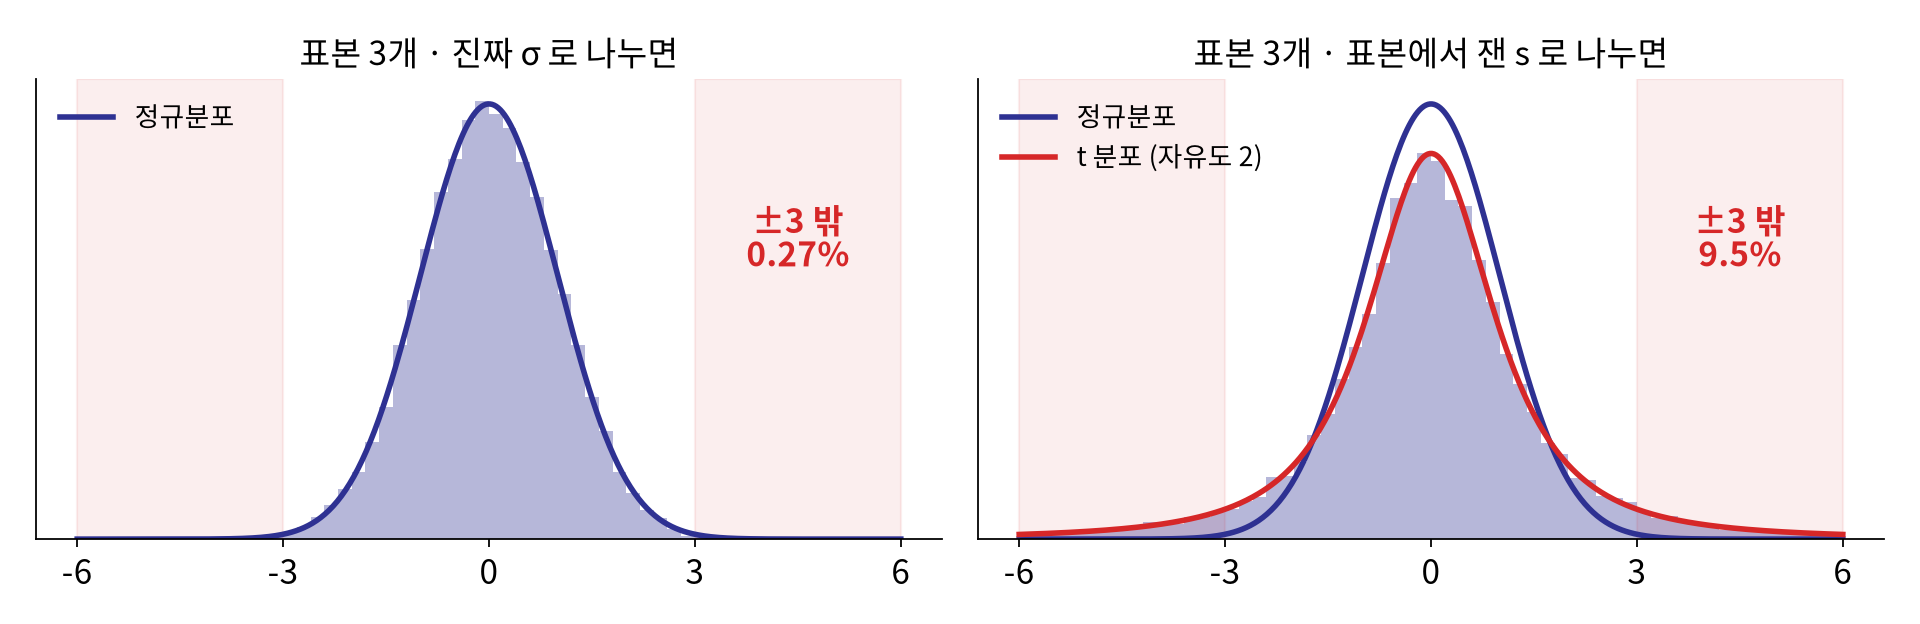
\includegraphics[width=0.9\linewidth]{ga_t_sim.png}\par\vskip0.2em
{\large 평균 $\bar x$ 를 표준화할 때 진짜 $\sigma$ 대신 \kq{표본에서 잰 $s$} 로 나누면 꼬리가 두꺼워진다}\\[0.2em]
{\small 정규분포에서 3개 뽑기를 2만 번 \quad $s$ 가 우연히 작으면 값이 크게 튄다 \quad 고셋 (Gosset), 가명 `Student'}
\vfill
\note{지금까지는 시그마를 안다고 생각했습니다. 그런데 표본이 아주 적으면 어떨까요? 1908년, 기네스 맥주 공장의 직원 고셋은 원료를 몇 개만 뽑아 검사해야 했습니다. 표본이 3개뿐이면 평균만 흔들리는 게 아니라, 퍼진 정도를 잰 값 s도 크게 흔들립니다. 그림은 정규분포에서 3개를 뽑는 일을 2만 번 반복한 결과입니다. 왼쪽처럼 진짜 시그마로 나누어 표준화하면 정규분포 그대로이고, 3 밖으로 벗어나는 경우는 0.27퍼센트뿐입니다. 오른쪽처럼 표본에서 잰 s로 나누면, s가 우연히 작게 나왔을 때 값이 크게 튀어서 꼬리가 두꺼워지고, 3 밖이 9.5퍼센트나 됩니다. 고셋은 회사 규정 때문에 스튜던트라는 가명으로 이 분포를 발표했습니다. 그래서 스튜던트 t 분포라고 부릅니다.}
\end{frame}

% --- t 분포 모양
\begin{frame}{스튜던트 t 분포: 가운데는 낮고, 꼬리는 두껍다}
\markpage{tdist}
\vfill
\centering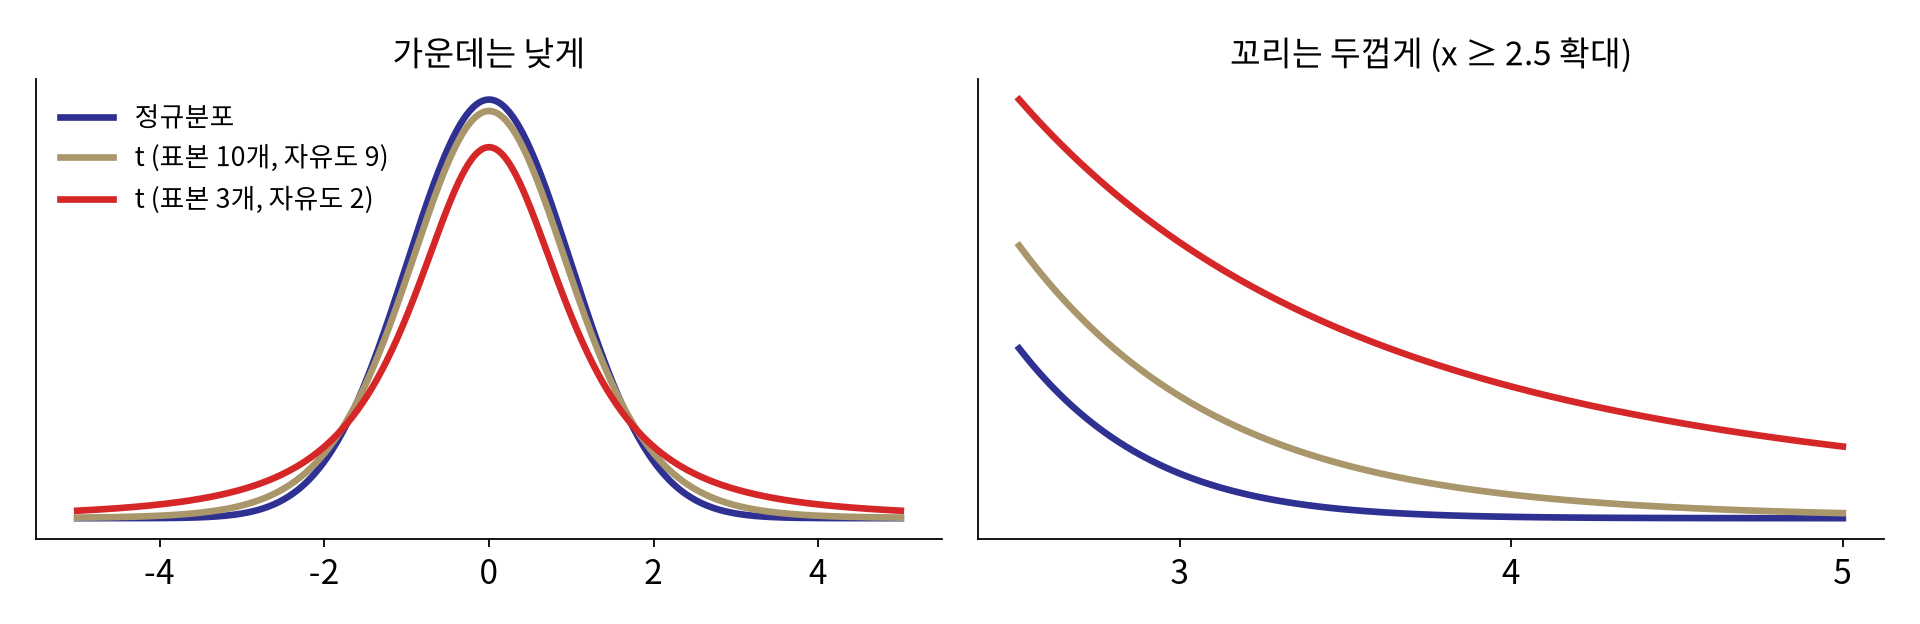
\includegraphics[width=0.76\linewidth]{ga_t_shape.png}\par\vskip-0.4em
{\Large $\displaystyle t = \frac{\bar x - \mu}{s / \sqrt{m}} \qquad s^2 = \frac{1}{m-1}\sum_{i=1}^{m}\big(x^{(i)} - \bar x\big)^2 \qquad \text{자유도} = m - 1$}\par\vskip0.4em
{\large $\pm 3$ 밖: \; 정규 \textbf{0.27\%} \quad t(자유도 2) \kq{9.5\%}} \qquad {\small $m-1$: 평균을 데이터로 정해서 하나 줄어든 수}
\vfill
\note{표본에서 잰 s로 표준화한 값 t가 따르는 분포가 스튜던트 t 분포입니다. 정규분포보다 가운데는 낮고 꼬리는 두껍습니다. 오른쪽에 꼬리를 확대했는데, 표본이 3개면 빨간 꼬리가 정규분포보다 훨씬 위에 있습니다. 평균에서 3 넘게 벗어날 확률이 정규분포는 0.27퍼센트, 표본 3개짜리 t 분포는 9.5퍼센트입니다. 여기서 s 제곱은 m이 아니라 m 빼기 1로 나눕니다. 평균을 데이터로 이미 정했기 때문에 자유롭게 움직일 수 있는 값이 하나 줄었다는 뜻이고, 이 m 빼기 1을 자유도라고 부릅니다. t 분포의 모양은 자유도 하나로 정해집니다. 참고로 데이터 지도를 그리는 t-SNE의 t도 이 분포입니다.}
\end{frame}

% --- 95% 구간
\begin{frame}{표본이 적으면 95\% 구간을 넓게}
\vfill
\begin{columns}[c]
\begin{column}{0.54\textwidth}\centering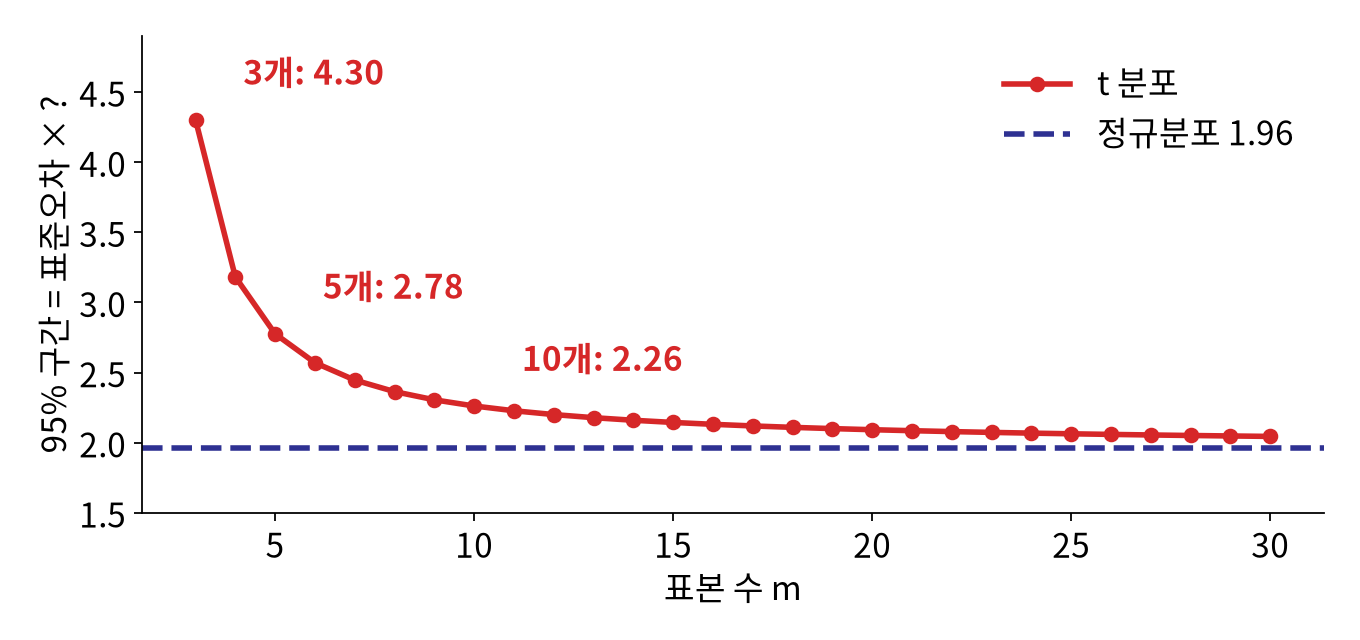
\includegraphics[width=\linewidth]{ga_t_crit.png}\end{column}
\begin{column}{0.44\textwidth}
{\large 키 5명 \pref{fit}: $\bar x = 174$}\\[0.3em]
$s^2 = \dfrac{80}{5-1} = 20$, \quad $s = 4.47$\\[0.3em]
표준오차 $\dfrac{s}{\sqrt{5}} = \dfrac{4.47}{2.24} = 2.0$\\[0.6em]
{\large 평균의 95\% 구간}\\[0.3em]
\textcolor{ksared}{t (자유도 4)}: $174 \pm 2.78 \times 2.0 = 174 \pm \mathbf{5.6}$\\[0.3em]
\textcolor{ksablue}{정규}: $174 \pm 1.96 \times 2.0 = 174 \pm 3.9$\\[0.6em]
{\small 표본이 늘면 t 분포 $\to$ 정규분포 (30개면 2.05)}
\end{column}
\end{columns}
\vfill
\note{t 분포가 실제로 쓰이는 곳은 신뢰구간입니다. 평균의 95퍼센트 구간은 표준오차에 어떤 배수를 곱해서 정하는데, 정규분포면 1.96배입니다. t 분포는 꼬리가 두꺼우니 더 넓혀야 합니다. 표본 3개면 4.30배, 5개면 2.78배, 10개면 2.26배이고, 표본이 늘수록 1.96에 가까워집니다. 30개면 2.05라서 거의 같습니다. 앞에서 본 키 5명 데이터로 해 봅시다. 평균은 174, s 제곱은 80을 4로 나눈 20, s는 4.47, 표준오차는 이것을 루트 5로 나눈 2.0입니다. t 분포를 쓰면 174 플러스마이너스 5.6, 정규분포를 쓰면 플러스마이너스 3.9입니다. 표본이 5개뿐이니, 정규분포로 계산하면 실제보다 너무 자신만만한 구간이 됩니다.}
\end{frame}

\section{푸아송}
% --- 푸아송 분포
\begin{frame}{푸아송 분포: 1분에 전화가 몇 통 올까?}
\markpage{poisson}
\vfill
\begin{columns}[c]
\begin{column}{0.52\textwidth}\centering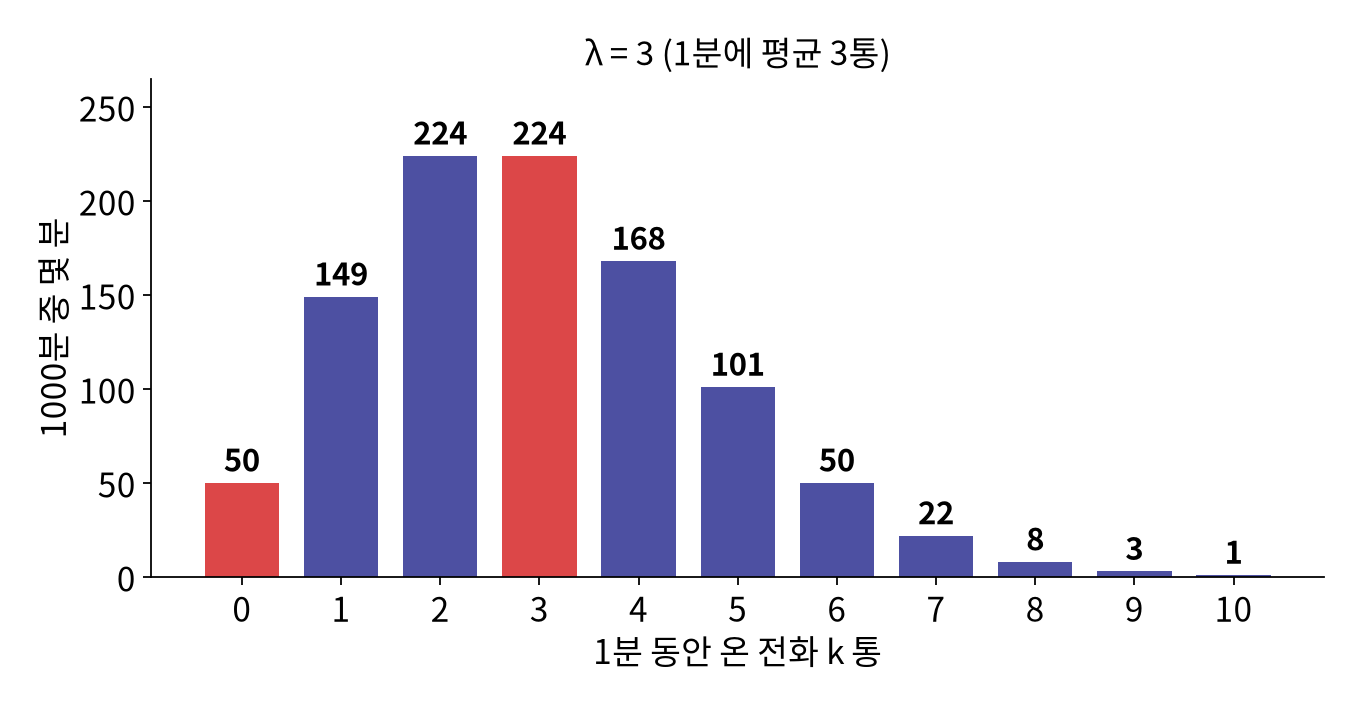
\includegraphics[width=\linewidth]{ga_poisson.png}\end{column}
\begin{column}{0.46\textwidth}
{\large 고객센터에 1분에 평균 \textbf{3통}}\\[0.4em]
{\LARGE $\displaystyle P(k) = \frac{\textcolor{ksablue}{\lambda}^{k}\, e^{-\textcolor{ksablue}{\lambda}}}{k!}$}\\[0.6em]
\textcolor{ksablue}{$\lambda$}: 평균 횟수 (rate) \quad $k$: 실제로 온 횟수\\[0.6em]
$P(0) = e^{-3} = 0.050$ \; $\to$ 1000분 중 \kq{50분}은 0통\\[0.3em]
$P(3) = \dfrac{3^3 e^{-3}}{3!} = 0.224$ \; $\to$ \kq{224분}\\[0.6em]
{\small 정해진 시간 · 공간에서 \textbf{드문 일이 몇 번} 일어나는지 (접속 수, 주문 수, 불량 개수)}
\end{column}
\end{columns}
\vfill
\note{지금까지는 키나 점수처럼 연속적인 값이었습니다. 이번에는 횟수를 세 봅니다. 어떤 고객센터에 1분에 평균 3통의 전화가 옵니다. 어떤 1분에는 한 통도 안 오고, 어떤 1분에는 6통이 옵니다. 1분 동안 k통이 올 확률은 람다의 k제곱 곱하기 e의 마이너스 람다 제곱을 k 팩토리얼로 나눈 식으로 주어지고, 이것을 푸아송 분포라고 합니다. 람다는 평균 횟수, 여기서는 3입니다. 한 통도 안 올 확률은 e의 마이너스 3제곱, 0.050이라서 1000분을 지켜보면 약 50분은 전화가 한 통도 없습니다. 정확히 3통 올 확률은 3의 세제곱 곱하기 e의 마이너스 3제곱을 3 팩토리얼로 나눈 0.224, 1000분 중 224분입니다. 그림의 막대가 1000분 동안 각 횟수가 나온 분의 수입니다. 웹사이트 접속 수, 가게 주문 수, 제품의 불량 개수처럼 정해진 시간이나 공간에서 드문 일이 몇 번 일어나는지 셀 때 씁니다.}
\end{frame}

% --- 푸아송 → 종 모양
\begin{frame}{$\lambda$ 가 커지면 푸아송도 종 모양}
\vfill
\centering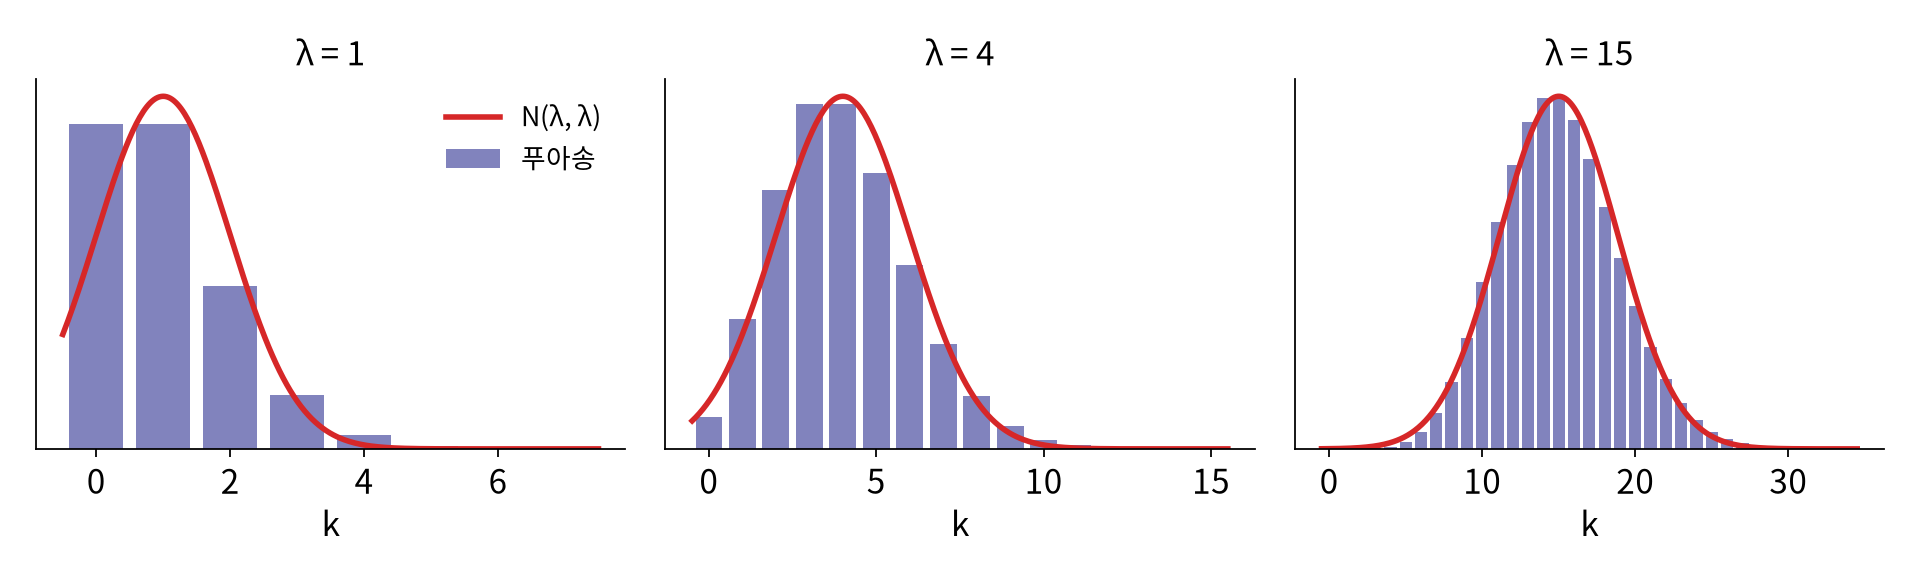
\includegraphics[width=0.94\linewidth]{ga_poisson_lam.png}\par\vskip0.3em
{\large 평균 $=$ 분산 $= \textcolor{ksablue}{\lambda}$ \qquad 데이터에서 $\hat\lambda =$ 평균 횟수 (MLE)}\\[0.3em]
{\large $\lambda$ 가 크면 $\approx \mathcal{N}(\lambda, \lambda)$}\\[0.3em]
{\small 1분 $=$ 60초, 매초 $\frac{3}{60}$ 확률로 오는 전화 60개의 합 $\to$ 골턴 보드처럼 작은 동전의 합 \pref{bins}}
\vfill
\note{푸아송 분포는 숫자 하나, 람다로 정해집니다. 평균도 람다, 분산도 람다입니다. 데이터에서 람다를 구할 때는 1분마다 온 횟수를 평균 내면 되고, 이것이 최대가능도 추정입니다. 그림은 람다가 1, 4, 15일 때입니다. 람다가 작으면 0 쪽으로 치우쳐 있지만, 커질수록 빨간 가우시안 곡선, 평균 람다 분산 람다인 종 모양과 거의 겹칩니다. 왜 그럴까요? 1분을 60초로 쪼개면, 매초 60분의 3 확률로 전화가 오는 동전 60개를 더한 것과 같습니다. 골턴 보드처럼 작은 동전을 많이 더한 것이니, 횟수가 커지면 종 모양이 됩니다.}
\end{frame}

\section{분류}
% --- 분류
\begin{frame}{종 두 개로 분류하기: 키 168 cm 는 남? 여?}
\markpage{heights}
\vfill
\centering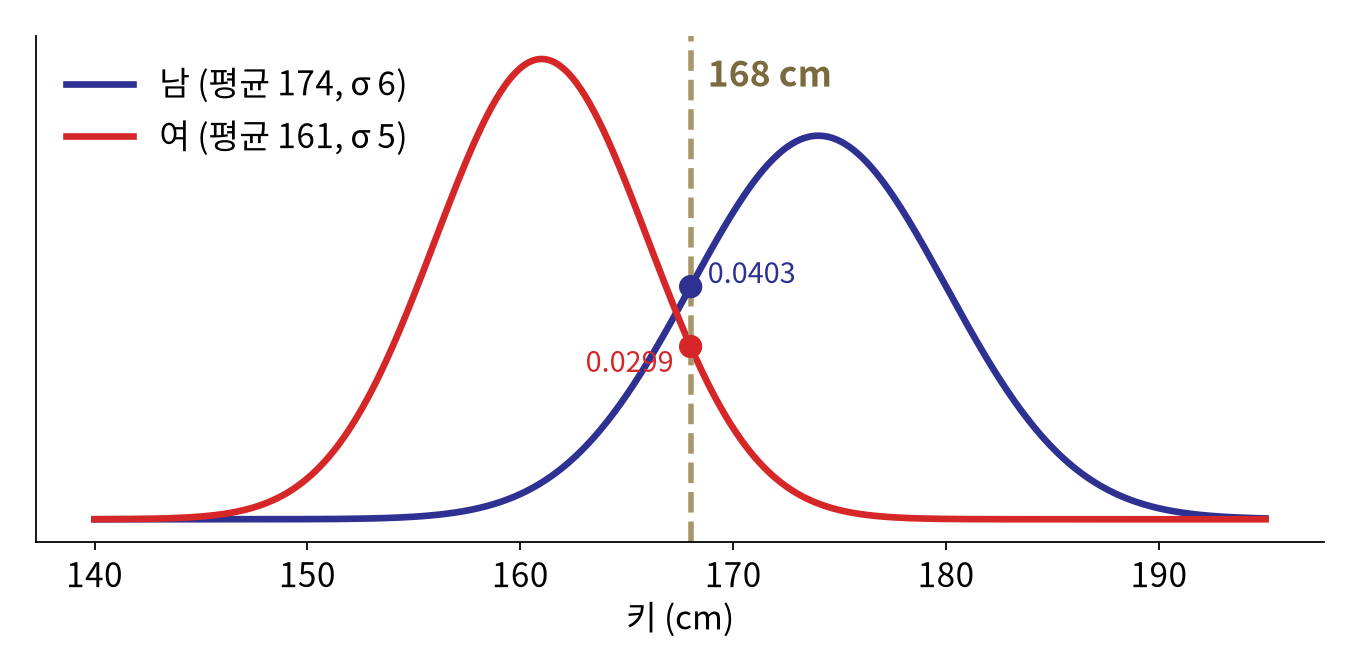
\includegraphics[width=0.62\linewidth]{ga_heights.png}\par\vskip0.2em
{\large 각 그룹의 키를 가우시안으로: \; 남 $\mathcal{N}(174, 6^2)$ \quad 여 $\mathcal{N}(161, 5^2)$ \quad (예시)}\\[0.2em]
{\large 168 cm 에서 종의 높이: \; \textcolor{ksablue}{남 0.0403} \quad \textcolor{ksared}{여 0.0299}}
\vfill
\note{이제 가우시안 분포로 분류를 해 봅니다. 남학생의 키를 평균 174, 표준편차 6인 가우시안으로, 여학생의 키를 평균 161, 표준편차 5인 가우시안으로 나타냈습니다. 예시 숫자입니다. 키가 168센티인 학생이 있습니다. 남일까요, 여일까요? 168에서 두 종의 높이를 읽으면 남은 0.0403, 여는 0.0299입니다. 이 높이가 남이라면 키 168이 나올 가능성이고, 가능도라고 부릅니다.}
\end{frame}

% --- 베이즈로
\begin{frame}{베이즈 정리로 확률까지}
\vfill
\centering
{\Large\[ \underbrace{P(\text{male}\mid 168)}_{\text{posterior}} = \frac{\textcolor{ksablue}{0.0403} \times \textcolor{ksared}{0.5}}{\underbrace{\textcolor{ksablue}{0.0403} \times \textcolor{ksared}{0.5} + \textcolor{ksablue}{0.0299} \times \textcolor{ksared}{0.5}}_{\text{evidence}}} = 0.57 \]}\vskip0.4em
\renewcommand{\arraystretch}{1.25}
{\normalsize\begin{tabular}{lll}
\textcolor{ksablue}{0.0403, 0.0299} & 가능도 likelihood & 남 · 여라면 168 cm 가 나올 정도 (종의 높이)\\
\textcolor{ksared}{0.5} & 사전확률 prior & 키를 보기 전 남 · 여일 확률 (반반 교실)\\
0.57 & 사후확률 posterior & 168 cm 를 본 뒤 남일 확률
\end{tabular}}
\vfill
\note{종의 높이를 베이즈 정리에 넣으면 확률이 나옵니다. 사전확률은 키를 보기 전 남일 확률, 반반 교실이라 0.5입니다. 분자는 남의 가능도 0.0403 곱하기 0.5, 분모는 남과 여 두 경우를 더한 것입니다. 계산하면 0.57, 168센티인 학생이 남일 확률은 57퍼센트입니다. 이 식이 베이즈 정리입니다. 왜 이렇게 되는지는 나이브 베이즈 시간에 메일 1000통을 직접 세며 자세히 봅니다. 거기서는 가능도를 단어를 세서 구하고, 오늘은 가우시안 종의 높이로 구한다는 점만 다릅니다.}
\end{frame}

% --- 경계
\begin{frame}{두 종이 만나는 곳이 경계}
\vfill
\centering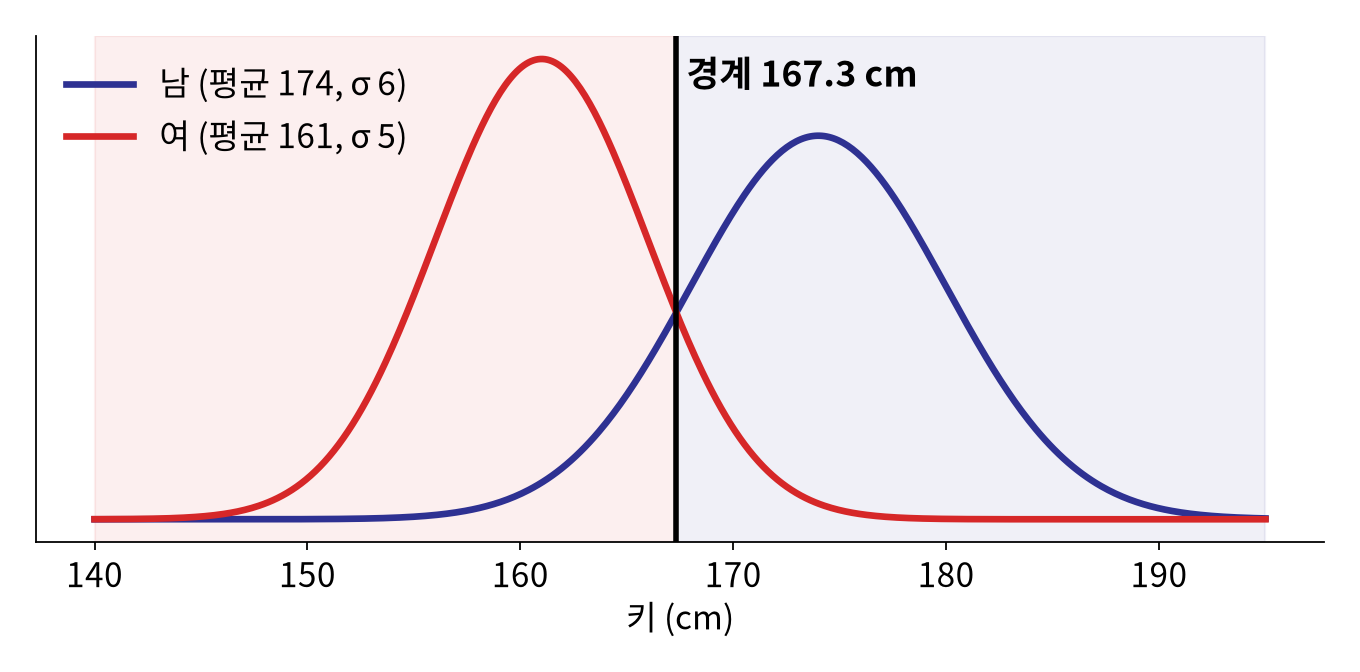
\includegraphics[width=0.6\linewidth]{ga_boundary.png}\par\vskip0.2em
{\large 사전확률이 반반이면 두 종의 높이가 같은 \kb{167.3 cm} 가 경계}\\[0.2em]
{\small $\sigma$ 가 다르면 경계가 둘일 수도 있다 (아주 멀리 가면 넓은 종이 다시 이긴다)}
\vfill
\note{어느 키에서 남과 여가 바뀔까요? 사전확률이 반반이면 두 종의 높이가 같은 곳, 167.3센티가 경계입니다. 그보다 크면 남, 작으면 여로 분류합니다. 하나 덧붙이면, 두 그룹의 표준편차가 다르면 경계가 두 개 생길 수도 있습니다. 아주 멀리 가면 더 넓게 퍼진 종이 다시 높아지기 때문입니다. 이렇게 그룹마다 가우시안을 맞추고 베이즈 정리로 분류하는 방법을 가우시안 판별분석, GDA라고 부릅니다.}
\end{frame}

% --- 사전확률
\begin{frame}{교실이 바뀌면: 사전확률}
\vfill
\centering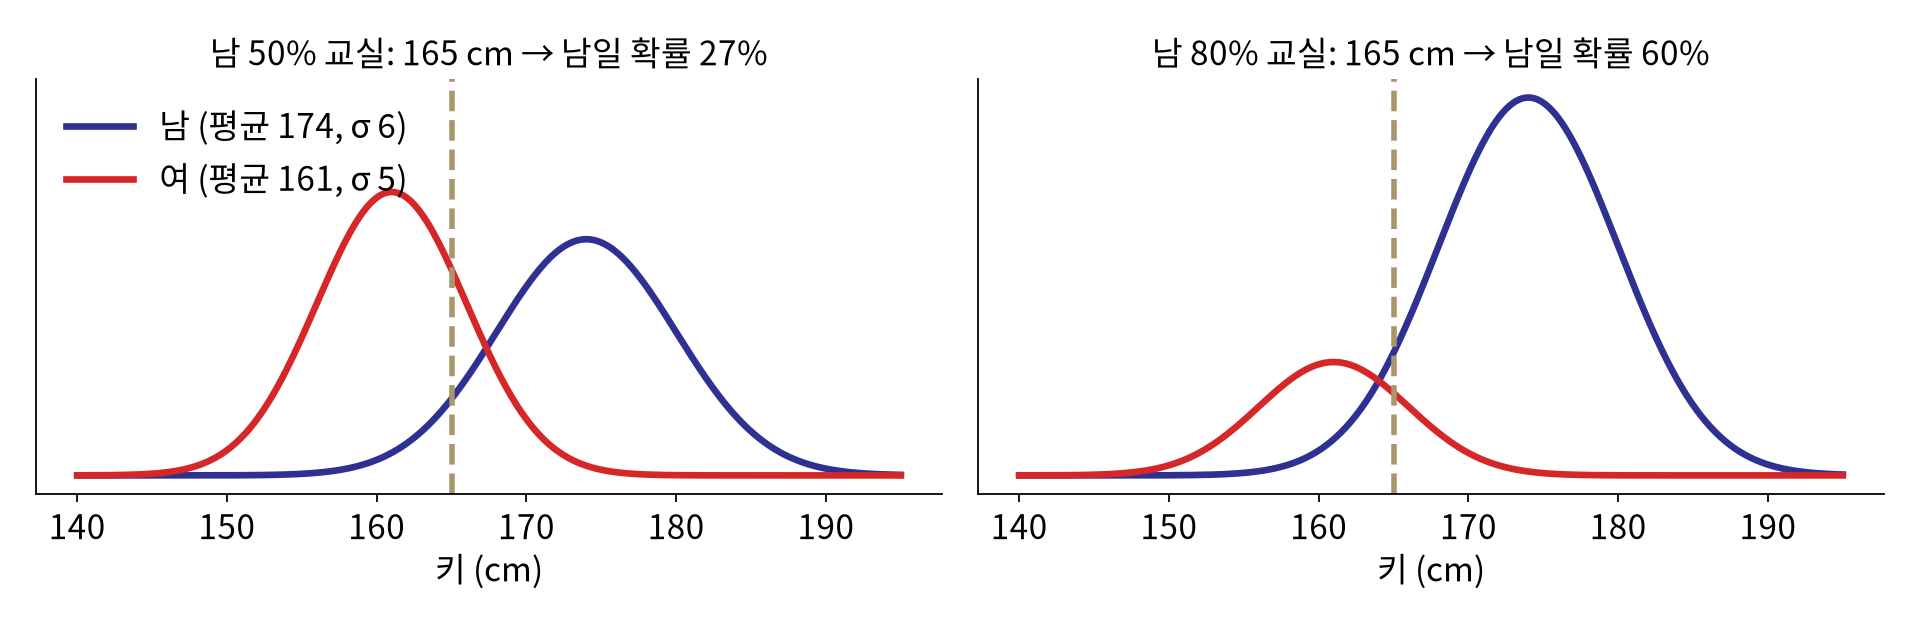
\includegraphics[width=0.92\linewidth]{ga_prior.png}\par\vskip0.2em
{\large 같은 165 cm 라도 \quad 남 50\% 교실 $\to$ 남일 확률 \textbf{27\%} \quad 남 80\% 교실 $\to$ \kq{60\%}}
\vfill
\note{같은 165센티라도 교실이 바뀌면 답이 바뀝니다. 남녀 반반 교실에서는 165센티인 학생이 남일 확률이 27퍼센트라서 여로 분류합니다. 그런데 남학생이 80퍼센트인 교실에서는 같은 키가 남일 확률 60퍼센트가 되어 남으로 분류합니다. 그림에서 남 종을 사전확률만큼 키우고 여 종을 줄였더니, 165센티에서 높이 순서가 뒤집혔습니다. 나이브 베이즈 시간에 스팸 메일함으로 이 사전확률의 힘을 다시 봅니다.}
\end{frame}

\section{연습}
% --- 문제풀이
\begin{frame}{문제풀이}
\vfill
\begin{enumerate}
\item 공 1000개, 못 10줄인 골턴 보드에서 오른쪽으로 정확히 2번 튀는 길은 몇 가지? 그 칸에 쌓이는 공은 약 몇 개?\vskip0.8em
\item 평균 70, 표준편차 10 인 시험. (a) 50 점 이하는 약 몇 \%? \; (b) 60 점과 80 점 사이는?\vskip0.8em
\item 데이터 2, 4, 6, 8 의 $\hat\mu$ 와 $\hat\sigma$ 는?\vskip0.8em
\item 3번 데이터로 평균의 95\% 구간을 t 분포로 (자유도 3 $\to$ 3.18). \; 정규 1.96 을 쓰면?\vskip0.8em
\item 1분에 평균 2통 오는 전화. 1분 동안 (a) 한 통도 안 올 확률은? \; (b) 정확히 2통 올 확률은? \; ($e^{-2} = 0.135$)\vskip0.8em
\item 남 · 여의 가능도가 0.02, 0.06 이고 남 75\% 교실이다. 남일 사후확률은?
\end{enumerate}
\vfill
\note{1번 답. 10개 중 2개를 고르는 경우의 수 45가지이고, 1000 곱하기 45 나누기 1024, 약 44개입니다. 2번 답. a는 z가 마이너스 2이니 아래쪽 꼬리, 약 2.3퍼센트, b는 평균에서 표준편차 1개 안이니 약 68퍼센트입니다. 3번 답. 평균은 5, 편차가 마이너스 3, 마이너스 1, 1, 3이라 제곱의 평균이 5, 시그마는 루트 5, 약 2.24입니다. 4번 답. s 제곱은 편차 제곱의 합 20을 4 빼기 1, 즉 3으로 나눈 6.67, s는 2.58, 표준오차는 이것을 루트 4, 즉 2로 나눈 1.29입니다. t 분포로는 5 플러스마이너스 3.18 곱하기 1.29, 약 5 플러스마이너스 4.1이고, 정규분포 1.96을 쓰면 5 플러스마이너스 2.5로 훨씬 좁습니다. 5번 답. 람다가 2인 푸아송 분포입니다. a는 e의 마이너스 2제곱, 0.135, 약 13.5퍼센트입니다. b는 2의 제곱 곱하기 e의 마이너스 2제곱을 2 팩토리얼로 나눈 0.271, 약 27퍼센트입니다. 6번 답. 0.02 곱하기 0.75는 0.015, 0.06 곱하기 0.25도 0.015라서 정확히 반반, 50퍼센트입니다.}
\end{frame}

% --- 실습
\begin{frame}{실습}
\vfill
\centering\begin{tabular}{rl}
\large 1 & 골턴 보드 시뮬레이션: 공 1000개 $\to$ 246 근처, 줄 수를 늘리며 종 모양 보기\\[0.5em]
\large 2 & 실제 데이터에 종 맞추기: 펭귄 3종의 날개 길이, $\hat\mu$ · $\hat\sigma$ 와 68\% 규칙 확인\\[0.5em]
\large 3 & 가우시안으로 분류: 날개 길이로 펭귄 종 맞히기, 사전확률 넣고 빼기
\end{tabular}\vskip1em
Palmer Penguins (Gorman et al., 2014) \\[0.4em]\href{https://colab.research.google.com/github/SuminHan/book-ml/blob/main/slides/v2/ml1/week03/gaussian/lab/gaussian.ipynb}{\textcolor{ksagolddk}{▶ Colab에서 실습 노트북 열기}}
\vfill
\note{실습은 세 부분입니다. 첫째, 골턴 보드를 시뮬레이션해서 공 1000개를 떨어뜨리고 가운데 칸이 246개 근처인지 확인합니다. 줄 수를 늘리면 종 모양이 어떻게 되는지도 봅니다. 둘째, 남극 펭귄 3종의 날개 길이 실제 데이터에 가우시안을 맞추고, 68퍼센트 규칙이 실제로 맞는지 셉니다. 셋째, 날개 길이 하나로 펭귄 종을 맞히는 가우시안 분류기를 직접 만들고, 사전확률을 넣을 때와 뺄 때를 비교합니다.}
\end{frame}

\section{정리}
% --- 정리
\begin{frame}{정리}
\vfill
\centering\large\begin{tabular}{l}
작은 효과가 많이 더해지면 \textbf{종 모양} = 가우시안 분포 (정규분포)\\[0.5em]
\textcolor{ksablue}{$\mu$} (위치) 와 \textcolor{ksared}{$\sigma$} (폭) 두 숫자로 정해진다 \quad $\pm1\sigma$ 68\%, $\pm2\sigma$ 95\%\\[0.5em]
데이터에서: $\hat\mu$ = 평균, $\hat\sigma^2$ = 평균에서 떨어진 거리 제곱의 평균\\[0.5em]
표본이 적으면 \textbf{스튜던트 t 분포}: 꼬리가 두꺼워 95\% 구간이 넓다 (자유도 $m-1$)\\[0.5em]
횟수를 세면 \textbf{푸아송 분포}: $\lambda$ 하나로 정해진다 (평균 $=$ 분산 $= \lambda$)\\[0.5em]
그룹마다 종을 맞추고 \textbf{베이즈 정리} $\to$ 분류 (가능도 = 종의 높이)
\end{tabular}
\vfill
\note{정리합니다. 작은 효과가 많이 더해지면 종 모양이 되고, 이것이 가우시안 분포입니다. 평균 뮤와 표준편차 시그마 두 숫자로 정해지고, 평균에서 시그마 1개 안에 68퍼센트, 2개 안에 95퍼센트가 들어옵니다. 데이터에서는 평균과, 평균에서 떨어진 거리 제곱의 평균으로 두 숫자를 구합니다. 표본이 적어서 표준편차까지 데이터로 재야 할 때는 꼬리가 두꺼운 스튜던트 t 분포를 쓰고, 그만큼 95퍼센트 구간을 넓게 잡습니다. 정해진 시간에 일이 몇 번 일어나는지 셀 때는 푸아송 분포를 쓰고, 평균 횟수 람다 하나로 정해집니다. 그룹마다 가우시안을 맞추면 종의 높이가 가능도가 되고, 베이즈 정리로 분류할 수 있습니다. 특징이 여러 개일 때는 지난주 나이브 베이즈가 그 방법이었습니다. 다음 시간부터는 라벨 없이 무리를 찾는 k-means와, 이 분포들을 섞는 EM 알고리즘으로 이어집니다.}
\end{frame}
\end{document}
